% vim: ft=tex expandtab

\documentclass[12pt]{report}
\usepackage[utf8]{inputenc}
\usepackage[serbian]{babel}
\usepackage[backend=biber, style=numeric, sorting=none]{biblatex}
\usepackage{csquotes}
\usepackage[a4paper, top=20mm, bottom=20mm, left=30mm, right=15mm, headheight=10mm, headsep=5mm, footskip=9mm]{geometry}
\usepackage{fancyhdr}
\usepackage{float}
\usepackage{fontspec}
\usepackage[acronym]{glossaries}
\usepackage{graphicx}
\usepackage{hyperref}
\usepackage{titlesec}
\usepackage{ragged2e}
\usepackage{setspace}

\hypersetup{hidelinks}

\setmainfont{Times New Roman}

\tolerance=1
\emergencystretch=\maxdimen
\hyphenpenalty=10000
\hbadness=10000

\addbibresource{literature.bib}

\pagestyle{fancy}

\renewcommand{\chaptermark}[1]{\markboth{#1}{}}
\renewcommand{\sectionmark}[1]{\markright{\arabic{section}.\ #1}}
\renewcommand{\baselinestretch}{1.4}
\newcommand{\normal}{
\tolerance=1
\emergencystretch=\maxdimen
}

\makeatletter
\newcommand\frontmatter{
    \cleardoublepage{}
    \pagenumbering{Roman}
    \setlength{\parskip}{0pt}
}

\setsansfont{Arial}

\newcommand\mainmatter{
    \cleardoublepage{}
    \pagenumbering{arabic}
    \setlength{\parskip}{2mm}
    \titleformat{\chapter}{\normalfont\Large\bf\sffamily\raggedleft}{\thechapter.}{12pt}{}
}
\makeatother

\titlespacing*{\chapter}{0mm}{58mm}{10mm}
\titleformat{\chapter}{\normalfont\Large\bf\sffamily}{\thechapter.}{12pt}{}
\titleformat{\section}{\normalfont\large\bf\sffamily}{\thesection}{12pt}{}
\titleformat{\subsection}{\normalfont\bf\sffamily}{\thesubsection}{12pt}{}
\titleformat{\subsubsection}{\normalfont\bf\sffamily}{\thesubsubsection}{12pt}{}
\setcounter{secnumdepth}{4}

\fancypagestyle{plain}{}
\fancyhead[L]{}
\fancyhead[R]{\leftmark}
\fancyfoot{}
\fancyfoot[R]{\thepage}

\raggedbottom{}

\begin{document}

\frontmatter{}

\renewcommand{\MakeUppercase}[1]{#1}
\tableofcontents

\listoffigures

\chapter*{Skraćenice}
\chaptermark{Skraćenice}
\begin{tabular}{ l l }
    \textbf{API} & -- \textit{Application programming interface}, Interfejs za programiranje aplikacija \\
    \textbf{URL} & -- \textit{Application programming interface}, Interfejs za programiranje aplikacija \\
    \textbf{CLI} & -- \textit{Application programming interface}, Interfejs za programiranje aplikacija \\
    \textbf{YAML} & -- \textit{Application programming interface}, Interfejs za programiranje aplikacija \\
    \textbf{GCC} & -- \textit{Application programming interface}, Interfejs za programiranje aplikacija \\
    \textbf{PDF} & -- \textit{Application programming interface}, Interfejs za programiranje aplikacija \\
\end{tabular}

\mainmatter{}
\chapter{Uvod}
U današnje vreme

\chapter{Teorijske osnove}
U ovom poglavlju će biti ukratko objašnjeni svi koncepti i alati koji su bili potrebni za izradu projekta o kojem ovaj rad govori. NABROJ
\section{Open source razvoj}
\section{Sistem za praćenje verzija datoteka}
Sistem za praćenje verzija datoteka (eng.\ \textit{version control system}) je sistem zadužen za praćenje istorije promena u datotekama. Promena koja se pamti se najčešće naziva revizija. Sve promene se uglavnom čuvaju na centralizovanom sistemu za skladištenje podataka i svi korisnici sa potrebnim privilegijama mogu da mu pristupaju, preuzmu najnoviju verziju datoteke ili grupe datoteka, izmene ih i zatim objave novu verziju koja se od tog momenta smatra najnovijom.

Pored najnovije verzije, čuva se i celokupna istorija promena i moguće je vratiti datoteke u bilo koju od prethodnih revizija. U poglegu softvera (eng.\ \textit{software}), ovo nam omogućava da vratimo u upotrebu bilo koju prethodnu verziju, u slučaju da dođe do greške u nekoj od novijih verzija. Istorija se čuvaju u strukturi tipa grafa:

\begin{figure}[H]
    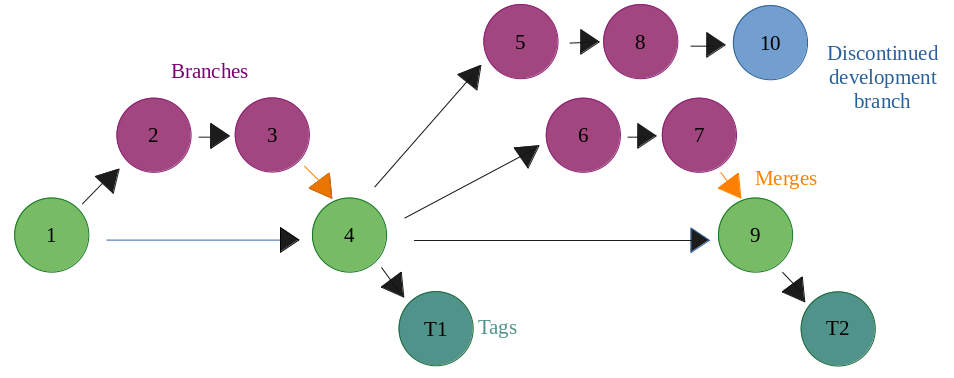
\includegraphics[width=\linewidth]{images/version_control.png}
    \caption{Sistem za praćenje verzija datoteka}
\end{figure}

Graf se najčešće sastoji od glavne grane(eng.\ \textit{branch}), na kojoj se nalaze glavne izmene, i pomoćnih grana na kojima se nalaze izmene za koje još nije odlučeno da li će pripadati glavnoj grani. Ako sve izmene na pomoćnim granama budu odgovarajuće, one se spajaju (eng.\ \textit{merge}) sa glavnom granom i postaju deo njenog sadržaja. U slučaju praćenja verzija softvera, ovakve grane najčešće predstavljaju nove funkcionalnosti (eng.\ \textit{feature}) koje se dodaju na glavnu granu projekta ili ispravljanje greške (eng.\ \textit{bugfix}) koja je nastala u nekoj od prethodnih verzija.

Važne izmene se mogu dodatno naglasiti dodavanjem oznake (eng.\ \textit{tag}). One uglavnom predstavljaju objavljivanje nove verzije softvera (eng.\ \textit{release}), dodavanje nove funkcionalnosti ili ispravku greške.

\section{Git}
Git \cite{git} je besplatan softver otvorenog koda (eng.\ \textit{open-source}) za praćenje verzija datoteka u distribuiranom okruženju. Primarno se koristi za razvoj softvera, ali se može koristiti i za praćenje bilo kojih drugih datoteka. Razvoj je započeo 2005. godine kreator Linux-a, Linus Torvalds, za potrebe razvoja jezgra Linux operativnog sistema. Distribuiran je pod GNU General Public License Version 2 licencom. Primarno je napravljen za Linux operativni sistem, ali je naknadno prilagođen i za macOS, BSD, Solaris i Windows.

Za razliku od drugih sistema za praćenje verzija datoteka u distribuiranom okruženju, Git nije softver klijent-server arhitekture. Svaki Git repozitorijum na svakom računaru čuva kompletnu istoriju promena i verzija i nije zavisan od pristupa mreži ili centralizovanom serveru. Kao takav, Git je osnova za razvoj mnogih drugih nezavisnih alata za praćenje verzija datoteka.

\section{GitHub}
GitHub \cite{github} je servis otvorenog koda za hostovanje (eng.\ \textit{hosting}) repozitorijuma sa različitim datotekama, najčešće izvornim kodovima za razna softverska rešenja. Za praćenje verzija datoteka, GitHub koristi Git. GitHub služi kao centralizovano mesto na kojem se čuvaju i razmenjuju sve izmene koje su sačuvane upotrebom Git alata.

U ovom trenutku, GitHub se smatra najpopularnijim alatom ovog tipa i trenutno broji preko 40 miliona korisnika. Stvari koje ovaj servis omogućava su:

\begin{enumerate}
    \item Upravljanje projektima
    \item Upravljanje timom
    \item Pregled i komentarisanje koda
    \item Integracija
    \item Paketi
    \item Bezbednost
    \item Hostovanje
    \item Akcije
\end{enumerate}

Moguće mu je pristupiti preko CLI verzije, desktop verzije, ekstenzije za Visual Studio program za uređivanje datoteka i mobilne aplikacije.

\subsection{Upravljanje projektima}
Upravljanje projektom je proces koji je potreban u bilo kojem većem programerskom projektu. Menadžeri projekta su zaduženi da prate razvoj projekta i upućuju programere u razvoj narednih delova projekata, kao i da upravljaju raspoređivanjem vremena rada na različitim zadacima koje projekat iziskuje.

GitHub nudi mogućnost koridinacije projektom, praćenje razvoja i menjanje statusa projekta na jednom mestu. Kordinacija započinje kreiranjem zadataka (eng.\ \textit{tasks}) koji traže izmene koda ili unapređenja projekta. Zadaci mogu biti u obliku greške/pitanja (eng.\ \textit{issue}), komentara (eng.\ \textit{comment}) ili pull-request-a, što podrazumeva kreiranje celine koja je spremna za spajanje sa glavnom granom na projektu. Zadacima se dodeljuju osobe koje su zadužene za njih. Time će oni dobijati obaveštenja kada dođe do bilo koje izmene u kodu vezane za njihov deo posla. Zadacima je moguće dodeliti i prioritet i oznake, što dodatno olakšava proces upravljanja projektom.

Sve ove informacije moguće je pratiti i menjati u formi tabele (eng.\ \textit{board}) ili u repozitorijumu na kojem se projekat nalazi. Svaki zadatak ima unikatan URL na kojem se mogu videti sve potrebne informacije vezane za njega. Čuva se i istorija svih zadataka i izmena na projektu, kojima se stvara uvid u proces razvoja projekta. Po završetku svih zadataka, urpavljanje projektom se završava i projekat se označava kao završen.

\subsection{Upravljanje timom}
Kako u timu imamo različite uloge, koje imaju različite permisije, GitHub nudi mogućnost hijerarhijskog organizovanja učesnika na projektu gde se svakoj grupi učesnika ili pojedincu dodeljuju potrebna prava.

Takođe, moguće je dodati u repozitorijum dokumente koji se tiču projekta, kao što su kodeks ponašanja (eng.\ \textit{code of conduct}) i licenca (eng.\ \textit{license}). Ove dokumente nije potrebno svaki put pisati iznova, već postoje unapred predefinisane verzije često korišćenih kodeksa ponašanja i licenci.

\subsection{Pregled i komentarisanje koda}
Komunikacija između učesnika na projektu doprinosi kvalitetu izrade samog projekta. Pored podele zadataka i raspoređivanja vremena za svaki zadatak, javlja se potreba i za diskutovanjem koda koji se dodaje u obliku pull-request-a.

Pri kreiranju pull-request-a, GitHub nudi prikaz svih izmena u odnosu na granu sa koje su izmene krenule i na koju bi se dodale ako je sve u redu. Taj prikaz je dostupan svima koji učestvuju u izradi projekta. Moguće je, dodatno, zamoliti nekoga od učesnika da pregleda izmene pre njihovog spajanja sa odabranom granom (eng.\ \textit{requests a review}). Na svakoj od izmena, moguće je dodati poruku, koja otvara mogućnost diskusije sa ostalim učesnicima projekta. Po zavšetku, osoba koja je zadužena da pregleda izmene može da odobri ili dobije pull-request, uz mogućnost traženja dodatnih izmena pre odobrenja.

Takođe, pri kreiranju pull-request-a, GitHub automatski pregleda kod u potrazi za bezbednosnim propustima ili konfliktima sa granom sa kojom se trenutna grana spaja. Ako ih ima, GitHub obaveštava korisnika i traži izmenu pre odobrenja i spajanja koda.

\subsection{Integracija}
Pored samog pisanja aplikacije, često se javlja potreba za testiranjem i pracenjem (eng.\ \textit{monitoring}) aplikacije, automatizovanim postavljanjem u produkciju (eng.\ \textit{deployment}), kontinualnom integracijom (eng.\ \textit{continuous integration}), proverom kvaliteta koda (eng.\ \textit{code quality}) i drugim pomocnim aktivnostima u procesu razvoja softver-a.

Pošto GitHub nije u mogućnosti da ponudi sve te aktivnosti, omogućio je proces integracije sa servisima koji ih nude. Svi ovi servisi mogu se pronaći u GitHub prodavnici (eng.\ \textit{marketplace}) \cite{marketplace}. Jedna od novina u GitHub prodavnici su GitHub akcije koje će biti jedna od centralnih tema ovog rada, a bice opisane u narednoj sekciji.

\subsection{Paketi}
Alati poput NPM-a, Docker-a, Maven-a, Gradle-a i drugih omogućavaju kreiranje artifakta koji sadrže sve potrebne alate za pokretanje nekog softverskog rešenja. Većina ovakvih servisa ima mogućnost čuvanja artifakta na njihovim repozitorijumima.

Zbog jednostavnosti korišćenja, GitHub je kreirao alat koji objedinjuje mnoge ovakve repozitorijume u jedan repozitorijum - GitHub Packages.

\subsection{Bezbednost}
Bezbednost u softverskim rešenjima igra veoma bitnu ulogu i najčešće zavisi od mnogo faktora: programera, ljudi koji održavaju kod (eng.\ \textit{maintainers}), istraživača, timova specijalizovanih za bezbednost i drugih. Da bi se postigao što veći stepen bezbednosti, potrebno je da što više različitih strana učestvuje u testiranju koda na bezbednosne propuste (eng.\ \textit{vulnerabilities}).

Neke od mogućnosti koje GitHub nudi za poboljšanje bezbednosti koda koji se nalazi na njemu su:

\begin{itemize}
    \item \textbf{Automatsko skeniranje koda} - pri dodavanju koda na repozitorijum, pokreće se automatsko skeniranje koda na poznate bezbednosne propuste i obaveštava se korisnika ako se pronađe neki od njih
    \item \textbf{Definisanje bezbednosnog procesa rada projekata otvorenog koda} - omogućava definisanje bezbednosnih polisa u okviru \textit{SECURITY.MD} datoteke u repozitorijumu u kojoj se navode sve potrebne informacije o tome koje bezbednosne probleme i na koji način treba da prijave korisnici koji ih pronađu
    \item \textbf{Diskutovanje o uticaju bezbednosnih propusta} - kada neki od korisnika prijavi bezbednosni propust ili grešku u kodu, GitHub nudi prostor za komentarisanje i razmenu mišljenja vezanih za postavljeni problem
    \item \textbf{Automatsko skeniranje zavisnosti} - slično skeniranju koda, pokreće se automatsko skeniranje zavisnosti nekog projekta - odnosno svih drugih softverskih rešenja od kojih projekat zavisi. Ako neko od njih ima bezbednosni propust, korisnik se obaveštava o tome. Ovakvi problemi često budu otklonjeni u narednoj verziji rešenja od kojeg projekat zavisi, pa GitHub često nudi promenu verzije kao rešenje ovakvog problema. Ovaj proces se nastavlja za vreme životnog ciklusa projekta, i ako se u bilo kojem momentu pronađe bezbednosni propust, automatski se kreira pull-request sa ispravkom
    \item \textbf{Pretraga kredencijala} - korisnicima se može desiti da slučajno upišu kredencijale za neki od eksternih servisa u kod projekta. Takvi kredencijali imaju specifičan oblik koji GitHub prepoznaje za preko 24 servisa i obaveštava korisnika ako ih pronađe
\end{itemize}

\subsection{Hostovanje sajtova}
Pored hostovanja repozitorijuma, što je glavna uloga GitHub-a, postoji i mogućnost hostovanja sajta pod GitHub domenom. Potrebno je napraviti repozitorijum sa nazivom \textit{username.github.io} i svi dokumenti u okviru njega će biti statički hostovani pod \textit{username.github.io} domenom.

\subsection{Akcije}
Kao što vidimo iz prethodnih sekcija, GitHub nudi mnoge mogućnosti pored njegove osnovne namene - praćenja verzija datoteka. Ipak, ako i te mogućnosti nisu dovoljne, postoji alat - GitHub Actions koji nudi mogućnost pisanja tokova posla (eng.\ \textit{workflow}) i reagovanje na mnoge događaje, tako da korisnik može, u specifičnom formatu, da definiše sve potrebne reakcije na događaje i pokrije slučajeve koje ostali GitHub alati ne pokrivaju. Ove akcije najčešće podrazumevaju automatizaciju, podešavanje i izvršavanje delova softverskih rešenja nakon nekog specifičng događaja.

\subsubsection{Događaji}
Neki od događaja na koje je moguće reagovati su:

\begin{itemize}
    \item \texttt{create} - pokreće se izvršavanje svaki put kada se kreira nova granu ili oznaka
    \item \texttt{delete} - pokreće se izvršavanje svaki put kada se obriše granu ili oznaka
    \item \texttt{fork} - pokreće se izvršavanje pri račvanju novog projekta iz trenutnog projekta
    \item \texttt{gollum} - pokreće se izvršavanje svaki put kada se kreira ili izmeni Wiki stranica
    \item \texttt{issues} - pokreće se izvršavanje svaki put kada se desi issue događaj. što podrazumeva otvaranje teme sa pitanjem, njenu izmenu, zatvaranje, brisanje, označavanje, itd.
    \item \texttt{issue\_comment} - pokreće se izvršavanje svaki put kada se doda, izmeni ili obriše komentar na otvorenom pitanju
    \item \texttt{label} - pokreće se izvršavanje svaki put kada se doda, izmeni ili obriše oznaka
    \item \texttt{milestone} - pokreće se izvršavanje svaki put kada se doda, izmeni ili obriše prekretnica u projektu
    \item \texttt{project} - pokreće se izvršavanje svaki put kada se desi project događaj, što podrazumeva kreiranje, izmenu, zatvaranje ili brisanje projekta
    \item \texttt{public} - pokreće se izvršavanje svaki put kada privatni repozitorijum postane javni
    \item \texttt{pull\_request} - pokreće se izvršavanje svaki put kada se desi pull\_request događaj. što podrazumeva otvaranje pull-request-a, izmenu, zatvaranje, brisanje, dodeljivanje, označavanje, sinhronizaciju, traženje pregledanja, itd.
    \item \texttt{pull\_request\_review} - pokreće se izvršavanje kada se izvrši, izmeni ili obriše pregledanje pull-request-a
    \item \texttt{pull\_request\_review\_comment} - pokreće se izvršavanje kada se kreira, izmeni ili obriše komentar na pregledanju pull-request-a
    \item \texttt{push} - pokreće se izvršavanje svaki put kada se doda novi kod na granu
    \item \texttt{registry\_package} - pokreće se izvršavanje svaki put kada se objavi ili izmeni paket
    \item \texttt{release} - pokreće se izvršavanje svaki put kada se desi release događaj, što podrazumeva kreiranje, objavljivanje, izmenu ili brisanje nove verzije projekta
\end{itemize}

Takođe, moguće je zakazati izvršavanje neke akcije navođenjem tačnog datuma i vremena izvršavanja ili zakazivanje izvršavanja na primer svake nedelje u određeno vreme. Za opisivanje vremena koristi se softverski alat Cron, koji je zadužen za planiranje i zakazivanje poslova na osnovu vremena (eng.\ \textit{time-based job scheduler}) na Unix operativnim sistemima.

Tokovi poslova se opisuju u YAML formatu. Događaji se opisuju u okviru \textit{on} sekcije, uz dodatak \textit{type} i \textit{branch} podsekcija ako ima potrebe. Na primer:

\begin{samepage}
    \begin{verbatim}
    on:
        pull_request:
            branches:
            - master
        release:
            types:
            - created
    \end{verbatim}
\end{samepage}

\subsubsection{Poslovi}

Nakon prepoznavanja događaja, pokreće se izvaršavanje jednog ili više poslova (eng.\ \textit{jobs}), gde se svaki od poslova može sastojati od jednog ili više koraka (eng.\ \textit{step}).

Za poslove se definiše na kojem operativnom sistemu treba da se izvrše. U ponudi su Windows Server 2019, Ubuntu 20.04, Ubuntu 18.04, Ubuntu 16.04 i macOS Catalina 10.15. Opciono se dodaje naziv posla, dodatni uslov pod kojim se izvršava, promenjive koje se preuimaju iz okruženja (eng.\ \textit{environment variables}), maksimalno vreme izvršavanja (eng.\ \textit{timeout}) i drugi parametri.

\subsubsection{Koraci}

Koraci su zaduženi za pokretanje komandi, pokretanje zadataka za podešavanje (eng.\ \textit{setup tasks}) ili pokretanje GitHub Akcija iz trenutnog repozitorijuma, nekog javnog repozitorijuma ili sa Docker registra (eng.\ \textit{registry}). Korak ne mora da ima akciju u sebi, ali svaka akcija koja se pokreće mora da se pokreće kao izolovani korak. Svaki korak se pokreće kao zaseban proces u okruženju pokretača (eng.\ \textit{runner}) i ima pristup svom okruženju i sistemu datoteka na kojem se pokreće. Ako ima potrebe, mogu postojati zasebni koraci koji se pokreću na početku i kraju posla, koji služe da pripreme okruženje pre početka izvršavanja i odrade završne aktivnosti na kraju izvršavanja.

Kao i posao, korak sadrži svoj unikatni id, naziv, uslov izvršavanja ako postoji, ulazne parametre, promenjive koje se preuzimaju iz okruženja, maksimalno vreme izvršavanja itd. Aktivnost koja se izvršava u toku koraka može se definisati na dva načina, upotrebom jednom od sledećih rezervisanih reči:

\begin{itemize}
    \item\texttt{uses} - u slučaju kada se koristi postojeća akcija, na ovom mestu se navodi putanja do akcije (u trenutnom repozitorijumu, nekom javnom repozitorijumu ili na Docker registru) i verzija akcije u oblliku: \texttt{path/name@version}.
    \item\texttt{run} - u slučaju kada se ne koristi postojeća akcija, već se definiše niz komandi u interfejsu komandne linije operativnog sistema. Moguće je imati više \texttt{run} komandi u okviru jednog koraka. Tada se svaka komanda pokreće kao odvojeni proces u jezgru operativnog sistema. Ako se pod jednom \texttt{run} sekcijom pokrene komanda u više linija, tada se sve komande pokreću u okviru jednog procesa. Komande se mogu pokretati u jednom od sledećih jezika komandne linije: bash, pwsh, python, sh, cmd, powershell.
\end{itemize}

\subsubsection{Kontekst okruženja}
Na osnovu konteksta okruženja, moguće je odlučivati o tome da li će se neki korak ili posao izvršiti. Za to postoji rezervisana reč \texttt{if}. Kontekst se nalazi u nekoliko objekata koji su nosioci različitih informacija i konteksta različitih delova toka posla. Neki od najčešće korišćenih su:

\begin{itemize}
    \item\texttt{github} - informacije o toku posla

    Primer: naziv akcije, putanja do akcije, id trenutnog posla koji se izvršava, koji korisnik je zaslužan za pokretanje akcije, koji korisnik je vlasnik repozitorijuma na kojem je pokrenuta akcija, grana ili oznaka na kojo se desilo pokretanje akcije, itd.
    \item\texttt{env} - sadrži promenjive koje se preuzimaju iz okruženja podešene u okviru toka posla, posla ili koraka.
    \item\texttt{job} - informacije o poslu koji se trenutno izvršava

    Primer: status posla, kontejner u kojem se posao izvršava, servisi koji su potrebni za izvršavanje posla, itd.
    \item\texttt{steps} - informacije o koraku koji se trenutno izvršava

    Primer: status koraka, vrednost izlaznih promenjivih, itd.
    \item\texttt{runner} - informacije o pokretaču trenutnog posla

    Primer: operativni sistem, putanja privremenog (eng.\ \textit{temporary}) direktorijuma, itd.
    \item\texttt{secrets} - sadrži promenjive koje se čuvaju kao tajne
    \item\texttt{needs} - dozvoljava pristup promenjivama koje su izlazne promenjive prethodnih poslova
\end{itemize}

\subsubsection{Pisanje akcija}
Neke od unapred definisanih akcija nudi GitHub, dok su druge napisane od strane zajednice koja ih koristi. Svako može da napiše akciju koji koristi za sebe ili da je podeli sa drugim korisnicima. Akcija se može pokretati direktno u okviru virtuelne mašine (eng.\ \textit{virtual machine}) ili u okviru Docker kontejnera. Mogu se definisati ulazni i izlazni parametri i promenjive koje se preuimaju iz okruženja.

Pri pisanju akcije potrebno je kreirati \textit{action.yml} ili \textit{action.yaml} dotatoku koja definiše sve informacije potrebne za izvršavanje akcije. Akcija može biti u obliku Docker kontejnera, ili opisana u JavaScript programskom jeziku. Takođe, postoje kompozitne akcije (eng.\ \textit{composite run steps action}) koje omogućavaju kombinovanje nekoliko koraka u jednu akciju.

\begin{itemize}
    \item\textbf{Docker akcije} - Docker kontejneri upakuju celokupno okruženje sa kodom GitHub akcije. Ovo čini dosta pouzdano rešenje, pozto korisnik ne mora da brine o verzijama i alatima. U kontejneru se instalira izabrana verzija operativnog sistema i svi potrebni alati, što ovakav način pisanja akcija čini pogodnim za sisteme koji moraju da se prilagode specifičnom okruženju. Mana ovog pristupa je to što je potrebno dosta vremena da se kreira i pokrene kontejner pa su ove akcije sporije od JavaScript akcija.
    \item\textbf{JavaScript akcije} - Ove akcije se pokreću direktno na računarima pokretačima, što pojednostavljuje pisanje koda akcija i znatno ubrzava njihovo izvršavanje. Da bi se mogle izvršavati na bilo kojem operativnom sistemu, ove akcije moraju biti napisane u čistom JavaScript-u.
\end{itemize}

Akcije napisane od strane pojedinaca mogu se objaviti u GitHub prodavnici i time postati dostupne svima za korišćenje. Da bi akcija bila spremna za objavljivanje, potrebno je da se ceo kod akcije i datoteke potrebne za njeno izvršavanje nalaze u jednom repozitorijumu. Taj repozitorijum ne sme ništa drugo da sadrži. Takođe, repozitorijum mora biti javan, da bi drugi korisnici mogli da mu pristupe. Potrebno je dodati oznaku na repozitorijum, koja predstavlja verziju akcije u GitHub prodavnici i zatim je objaviti.

\subsubsection{Hostovanje pokretača}
GitHub nudi mašina koje hostuju pokretače GitHub Akcija, ali i daje mogućnost hostovanja akcija na korisničkom hardveru (eng.\ \textit{hardware}). Hostovanje na korisničkim mašinama daje veću slobodu korisnicima u izboru samih hardverskih komponenti, operativnog sistema i alata koji se instaliraju na tim mašinama. Mogu biti u obliku fizičkih mašina, virtuelnih mašina, kontejnera, ili računari u oblaku (eng.\ \textit{cloud}).

Korisničke mašine se povezuju sa GitHub-om preko aplikacije koju GitHub nudi. Ako se ne pokrene ni jedna akcija u roku od 30 dana, prekida se veza između korisničkog računara i GitHub-a.

Problem pri hostovanju na korisničkim mašinama može biti to što je korisnik zadužen za ažuriranje verzije operativnog sistema i svih softverskih alata na njemu, dok na GitHub-ovim mašinama to radi sam GitHub. Takođe, Githab pokreće novu, čistu instancu za svaki posao koji se izvršava, dok korisnik to ne mora da radi.

\section{Docker? opet ga svuda ima}
\section{Python}

Python \cite{python} je programski jezik opšte namene, spada u grupu programskih jezika visokog nivoa i interpretira se. Dizajniran je tako da bude izrazito čitljiv, što se postiže velikom upotrebom belina (eng.\ \textit{whitespace character}). Pogodan je za razvoj različitih projekata pošto podržava više programskih paradigmi:

\begin{enumerate}
    \item Proceduralnu
    \item Objektno orijentisanu
    \item Funkcionalnu
    \item Strukturalnu paradigmu
\end{enumerate}

Takođe, prilagođen je za korišćenje u radličitim okruženjima na različitim operativnim sistemima.

Python se prvi put spominje krajem 1980-tih kao naslednik ABC programskih jezika. Dizajnirao ga je Guido van Rossum i objavio prvu verziju 1991. godine. Python 2.0, koji je izdat 2000. godine je znatno unapređenje prve verzije, koje se do skoro koristilo.  Poslednja velika revizija urađena je 2008. godine kada je nastao Python 3.0. Zbog toga što Python 3 nije u potpunosti kompatibilan sa prethodnim verzijama, podrška za Python prestala je u januru 2020. godine.

Umesto da poseduje svu svoju funkcionalnost u jezgru OS-a. Python je dizajniran tako da  bude veoma proširiv, što ga je učinilo veoma pogodnim za dodavanje programabilnih interfejsa postojećim aplikacijama.

\section{Python paketi, PyPI}

Python paketi su imenski prostori (eng.\ \textit{namespaces}) koji u sebi sadrže druge pakete i module - delove softvera koji obavljaju konkretnu funkcionalnost. Svaki paket je direktorijum koji u sebi mora imati \textit{\_\_init\_\_.py} datoteku. Ova datoteka može biti prazna, što označava da je trenutni direktorijum Python paket i da može biti korišćen kao zaseban modul. Inače, \textit{\_\_init\_\_.py} datoteka čuva kod koji služi za inicijaliciju tog paketa.

Da bi se koristile funkcionalnosti koje neki paket nudi, potrebno ga je uvezati (eng.\ \textit{import}) u projekat korišćenjem rezervisane reči \texttt{import}. Da bi se uvezao pojedinačni modul iz nekog paketa, treba naznačiti koji modul se iz kojeg paketa uvezuje korišćenjem sledećeg Python koda:

\begin{itemize}
    \item \texttt{from <package> import <module>}
\end{itemize}

\subsection{Distribuiranje Python paketa}

Glavna uloga Python paketa je distribuiranje biblioteka za Python programski jezik. Paket može da kreira bilo ko i da ga potom podeli sa ostatkom Python zajednice. Da bi paket bio dostupan, potrebno je kreirati arhivu sa svim potrebnim konfiguracijama za njega i objaviti je na nekom repozitorijumu za Python pakete.

Repozitorijumi su softverski alati za čuvanje i distribuiranje paketa. Postoje javni repozitorijumi, koji omogućavaju razmenu paketa sa bilo kim, i privatni, koji omogućavaju razmenu paketa u ograničenoj grupi korisnika koji imaju specijalne privilegije.

Najčešće korišćen javni repozitorijum je PyPI \cite{pypi}  - The Python Package Index.

\section{Poetry}
Poetry \cite{poetry} je alat otvorenog koda za kreiranje Python paketa i upravljanje paketima koje Python projekat koristi(eng.\ \textit{dependency management}). Pomaže korisnicima tako što umesto njih instalira i menja verzije  bibliotekama od kojih projekat zavisi, a koje korisnik mora pretkodno da specificira. Poetry je takođe znatno olakšao kreiranje, pakovanje i objavljivanje paketa na PyPI repozitorijumu i time omogućio lakše deljenje Python projekata sa drugim korisnicima Python programskog jezika.

Prva verzija alata objavljena je 28.02.2018. godine. Verzije programskog jezika Python koje su podržane su 2.7 i 3.4+. Ideja je da Poetry radi podjednako dobro na različitim platformama, između ostalog na Linux-u, Windows-u i OSX-u.

\subsection{Podešavanje Poetry-ja}
Za razliku od drugih Python alata za upravljanje paketima od kojih projekat zavisi, umesto pip-a - instalera za Python pakete, Poetry koristi svoj specifičan način za instalaciju. Instalator doda Poetry u korisnički direktorijum, tako da može da se koristi sa bilo kojom verzijom Python-a. Omogućena je i instalacija Poetry-ja korišćenjem pip-a, ali se ne proporučuje iz dva razloga:

\begin{enumerate}
    \item može dovesti do konflikta sa drugim sistemskim fajlovima
    \item otežava održavanje konzistentnosti pre korišćenju različitih verzija Python-a i različitih virtuelnih okruženja (eng.\ \textit{virtual environments})
\end{enumerate}

\subsection{Kreiranje Python projekta koji koristi Poetry}
Nakon isntalacije alata, moguće je kreirati projekat koji koristi Poetry za upravljanje paketima ili dodati Poetry u postojeći projekat i time kreirati virtuelno okruženje u kojem će se izvršavati naredne akcije. U oba slučaja će se kreirati \textit{pyproject.toml} datoteka koja čuva sve bitne informacije o projektu. U početku ova datoteka sadrži samo osnovne informacije o projektu:

\begin{samepage}
    \begin{verbatim}
    [tool.poetry]
    name = "poetry-demo"
    version = "0.1.0"
    description = ""
    authors = ["Name Surname <email>"]

    [tool.poetry.dependencies]
    python = "*"

    [tool.poetry.dev-dependencies]
    pytest = "^3.4"
    \end{verbatim}
\end{samepage}

Informacije o samom projektu, njegovom autoru, verziji, licenci, opisu, dokumentaciji, itd. nalaze se u prvom segmentu - \texttt{[tool.poetry]}. Informacije o paketima koje projekat koristi nalaze se u naredne dve sekcije - \texttt{[tool.poetry.dependencies]} i \texttt{[tool.poetry.dev-dependencies]}, gde se u prvoj od ove dve sekcije nalaze informacije o paketima koji se koriste u produkcionom okruženju, a u drogoj informacije o paketima koji se koriste u toku razvoja projekta. Pri instalaciji novog paketa, njegov naziv i verzija će se dopisati u jednu od ove dve sekcije, ili u obe ako je to potrebno.

Ovu datoteku je moguće ručno menjati, ali se sa njom najčešće interaguje pozivanjem poetry komandi u konzoli. Neke od tih komandi su:

\begin{itemize}
    \item \texttt{poetry add} - dodaje novi paket u \textit{pyproject.toml} datoteku
    \item \texttt{poetry remove} - briše paket iz projekta
\end{itemize}

Komande koje takođe interaguju sa \textit{pyproject.toml} datotekom, ali je ne menjaju su:

\begin{itemize}
    \item \texttt{poetry install} - instalira pakete definisane u \textit{pyproject.toml} datoteci
    \item \texttt{poetry update} - ažurira pakete u skladu sa verzijama koje pišu u \textit{pyproject.toml} datoteci
    \item \texttt{poetry lock} - zaključava pakete u prijektu
    \item \texttt{poetry check} - proverava ispravnost \textit{pyproject.toml} datoteke
\end{itemize}

Za pokretanje komandi u virtuelnom okruženju opsisanom u \textit{pyproject.toml} datoteci koristi se komanda:

\begin{itemize}
    \item \texttt{poetry run}
\end{itemize}

Za sve ostale detalje najbolje je pogledati dokumentaciju pomoću komande:

\begin{itemize}
    \item \texttt{poetry help}
\end{itemize}

\subsection{Kreiranje, pakovanje i objavljivanje Python paketa}
Da bi se Python projekat mogao objaviti, potrebno je kreirati arhivu sa svim potrebnim konfiguracijama za njega. To se postiže upotrebom komande:

\begin{itemize}
    \item \texttt{poetry build}
\end{itemize}

Nakon toga, paket je spreman za objavljivanje. U projektu se pojavi novi direktorijum sa nazivom \texttt{dist} i u njemu se nalaze dve datoteke:

\begin{enumerate}
    \item \texttt{poetry-demo-0.1.0-py2.py3-none-any.whl}
    \item \texttt{poetry-demo-0.1.0.tar.gz}
\end{enumerate}

Repozitorijum na kojem se paket objavljuje se podešava pomoću komande:

\begin{itemize}
    \item \texttt{poetry config}
\end{itemize}

Paket se objavljuje pozivanjem komande:

\begin{itemize}
    \item \texttt{poetry publish}
\end{itemize}

U tom momentu, paket postaje dostupan na izabranom repozitorijumu i svako ko ima pristup repozitorijumu može da instalira paket. Najčešće se paketi objavljuju na PyPI repozitorijumu.

\section{Bash}

\chapter{Specifikacija i implementacija projekta}

Projekat o kojem ovaj rad govori sastoji se iz grupe alata koje je bilo potrebno napraviti i povezati da bi se dodale nove funkcionalnosti u postojeći projekat - \textit{pjisp-assignment-template} \cite{pjisp-assignment-template}. Pomenuti alat služi za automatizovano kreiranje studentskih zadataka, nihovo puštanje u učionicama u kojima studenti rade zadatke i na kraju pregledanje zadataka. Prvenstveno je namenjen da profesorima i asistentima olakša ceo proces od kreiranja do pregledanja kolokvijuma ili zadataka koje studenti rade.

Zadatak nastavnog osoblja je pre svega da iz repozitorijuma projekta koji je šablonski (eng.\ \textit{template}) repozitorijum kreira svoj repozitorijum sa zadatkom. Važno je da nastavnik svoj repozitorijum nazove u skladu sa predefinisanim načinom imenovanja. Nakon toga se u repozitorijumu kreiraju svi potrebni materijali koji su potrebni za generisanje studentskog zadatka. Zadatak nastavnika je da pokrenje generisanje zadatka za jedan od predefinisanih testova na predmetu Programski jezici i strukture podataka. Ovaj projekat dodaje mogućnost automatizovanog kreiranja zadatka za određeni test na osnovu naziva repozitorijuma koji nastavnik napravi uz proveru ispravnosti naziva.

Po završetku pisanja zadatka i njegovog testiranja, nastavnik, a najčešće asistent, je dužan da obavesti profesora o tome, da bi profesor mogao da proveri ispravnost zadatka i odobri korišćenje zadatka u nastavi ako je dobar i pogodan za studente. Kao olakšicu, nastavnik može da pokrene alat za testiranje zadatka i proveri ispravnost. Ovaj projekat uvodi isto to testiranje i nakon objavljivanja nove verzije zadatka na GitHub-u. Kao dodatnu proveru, jedan od alata iz ovog projekta proverava da li su izmenjene sve potrebne datoteke, da bi zadatak bio kompletan, odnosno da bi imao korektan tekst zadatka, primer rešenja i testove. Ako svi ovi alati vrate rezultat pozitivnog ishoda, u GitHub repozitorijumu se pojavljuje oznaka da su svi uslovi ispunjeni i da je zadatak spreman za pregledanje. U suprotnom, stoji oznaka da zadatak ne ispunjava sve potrebne uslove.

Naredna poglavlja opisuju alate koji su korišćeni da bi se postigla opisana unapređenja \textit{pjisp-assignment-template} alata, a poslednje poglavlje opisuje njihovu integraciju u jednu celinu.

\section{pjisp-template-name}
Alat \textit{pjisp-template-name} \cite{pjisp-template-name} je konzolna aplikacija kola služi za proveru ispravnosti naziva repozitorijuma. Napisana je u obliku konzolne aplikacije otvorenog koda u programskom jeziku Python.

\subsection{Način imenovanja repozitorijuma}
Za imenovanje repozitorijuma koristi se predefinisani šablon, koji izgleda ovako:

\begin{verbatim}
pjisp-{SCHOOL_YEAR}-{COURSE_ID}-{TEST_ID}-{GROUP_ID}
\end{verbatim}

gde su:

\begin{itemize}
    \item \texttt{{SCHOOL\_YEAR}} - školska godina, na primer 2019
    \item \texttt{{COURSE\_ID}} - identifikator kursa (E214 za zimski semestar ili E111 za letnji)
    \item \texttt{{TEST\_ID}} - identifikator testa (T12, T34 ili SOV)
    \item \texttt{{GROUP\_ID}} - identifikator grupe studenata, na primer G10
\end{itemize}

Alat pre svega proverava da li je dužina naziva ispravna, odnosno da li naziv ima sve celine odvojene znakom \textit{-}. Ako nema, ispisuje se poruke \textit{``Repository name length not valid''} i program izlazi sa izlaznim kodom \textit{1}. U suprotnom, program nastavlja sa izvršavanjem.

Nakon provere dužine, proverava se ispravnost ostalih tokena, prema malopre opisanom načinu davanja imena. Ako bilo gde dođe do greške, ispisuje se poruka  \textit{``Repository name not valid. Error on <token>''} i izlase se sa izlaznim kodom \textit{1}. Ako naziv u potpunosti ispunjava šablon, kao izlazna vrednost vraća se identifikator testa, da bi na osnovu toga mogle da se generišu datoteke potrebne za kreiranje tog testa.

\subsection{Instalacija i pokretanje}
Ovaj alat se instalira kao bilo koji drugi Python paket. Potrebno je u konzolnoj liniji pokrenuti komandu:

\begin{verbatim}
pip install pjisp-template-name
\end{verbatim}

i nakon toga je alat spreman za upotrebu. Pokreće se pozivanjem komande:

\begin{verbatim}
pjisp_template_name <template_name>
\end{verbatim}

\section{pjisp-diff}

Alat \textit{pjisp-diff} \cite{pjisp-diff} je konzolna aplikacija kola služi pomoćni alat nastavnicima koji proverava da li su izmenili sve potrebne datoteke pri kreiranju zadataka za studente. Napisana je u obliku konzolne aplikacije otvorenog koda u programskom jeziku Python.

Pored provere da li su promenjene sve potrebne datoteke, ovaj alat proverava i da li su ostale nepromenjene sve pomoćne datoteke koje nije potrebno menjati. Datoteke koje je potrebno menjati zavise od ulaznog parametra, šablona spram kojeg se kreira zadatak. Datoteke koje je potrebno uvek menjati su:

\begin{itemize}
    \item \texttt{assignment\_solution.c}
    \item \texttt{assignment.rst}
\end{itemize}

Ako je vrednost ulaznog parametra jednaka ``T12'', potrebno je menjati:

\begin{itemize}
    \item \texttt{fixtures/stdio-numbers.yaml}
\end{itemize}

Ako je šablon vrednost ulaznog parametra jednaka ``T34'' ili ``SOV'', potrebno je menjati:

\begin{itemize}
    \item \texttt{fixtures/file-error-input-not-readable.yaml}
    \item \texttt{fixtures/file-error-output-not-writable.yaml}
    \item \texttt{fixtures/fixtures/file-text.yaml}
\end{itemize}

Datoteka koju nije dozvoljeno menjati je:

\begin{itemize}
    \item \texttt{assignment\_notes.rst}
\end{itemize}

Ako su po završetku programa izmenjene sve potrebne datiteke i nisu izmenjene one koje ne smeju da se menjaju, alat vraća \textit{0} kao vrednost izlaznog koda. U suprotnom, alat vraća vrednost \textit{1} uz jednu ili više poruka u obliku: \textit{``Please change the <filename> file.''} ili \textit{``Please do not change the <filename> file.''}

\subsection{Instalacija i pokretanje}
Ovaj alat se instalira kao bilo koji drugi Python paket. Potrebno je u konzolnoj liniji pokrenuti komandu:

\begin{verbatim}
pip install pjisp-diff
\end{verbatim}

i nakon toga je alat spreman za upotrebu. Pokreće se pozivanjem komande:

\begin{verbatim}
pjisp_diff <template>
\end{verbatim}

gde \texttt{<template>} može biti T12, T34 ili SOV.

\section{poetry-publish}
Alati koji su opisani u prethodna 2 poglavlja napravljeni su tako da mogu biti instalirani i korišćeni kao Python paketi. Oba paketa su dostupna na PyPI repozitorijumu Python paketa. Za postavljanje na repozitorijum, korišćen je alat Poetry. Pošto je potrebno objaviti novu verziju paketa na repozitorijumu nakon svake izmene u samom paketu, korišćena je \textit{poetry-publish} \cite{poetry-publish-repo} GitHub akcija koja pri svakom novom objavljivanju verzije alata na GitHub-u, kreira i novu verziju Python paketa i postavlja je na PyPI repozitorijum.

Akcija \textit{poetry-publish} je kreirana od strane autora ovog rada pre nego što se razvila ideja za projekat koji je u ovom radu opisan, ali je znatno olakšala kreiranje malopre pomenutih paketa, tako da je imala veoma važnu ulogu i u ovom projektu. Akcija je projekat otvorenog koda i dostupna je za preuzimanje u GitHub prodavnici \cite{poetry-publish-marketplace}. Dostupna je pod BSD 3-Clause licencom.

\textit{poetry-publish} je GitHub akcija koja služi za kreiranje paketa i njihovo objavljivanje na Python repozitorijumu upotrebom alata Poetry. Kreirana je u obliku Docker akcije. U Docker kontejneru se instaliraju svi potrebni alati za korišćenje Python-a i zatim se pokrenu Poetry komande za kreiranje i objavljivanje paketa:

\begin{itemize}
    \item \texttt{poetry build} - da kreira Python paket
    \item \texttt{poetry publish} - da objavi paket na repozitorijumu koji je prethodno podešen
\end{itemize}

Paramtri koje ova akcija očekuje su:

\begin{itemize}
    \item \textbf{python\_version} - verzija Python-a koja se instalira u kontejneru i koristi za kreiranje paketa. Ako se ne navede, podrazumeva se da se koristi najnovija verzija. Za bolje performanse, poželjno je koristiti predefinisanu-najnoviju verziju.
    \item \textbf{poetry\_version} - verzija Poetry-a koja se instalira u kontejneru i koristi za kreiranje paketa. Ako se ne navede, podrazumeva se da se koristi najnovija verzija. Navodi se u PIP sintaksi za specifikaciju verzija
    \item \textbf{pypi\_token} - jedini obavezan parametar. Služi kao API token za autentifikaciju pri objavljivanju paketa na PyPI.
    \item \textbf{repository\_name} - naziv repozitorijuma na kojem se objavljuje paket. Ako se ne navede, podrazumeva se da se objavljuje na PyPI repozitorijumu. Potrebno je izmeniti pri objavljivanju na PyPI test repozitorijumu ili na privatnom repozitorijumu.
    \item \textbf{repository\_url} - adresa repozitorijuma na kojem se objavljuje paket. Ako se ne navede, podrazumeva se da se objavljuje na PyPI repozitorijumu. Potrebno je izmeniti pri objavljivanju na PyPI test repozitorijumu ili na privatnom repozitorijumu.
\end{itemize}

Takođe, potrebno je specificirati \textit{pyproject.toml} datoteku na osnovu koje će se kreirati Python paket. Ova datoteka treba da se nalazi u korenskom direktorijumu repozitorijuma koji koristi ovu akciju.

\subsection{Primer koraka koji koristi akciju}

\begin{verbatim}
- name: Build and publish to pypi
uses: JRubics/poetry-publish@v1
with:
    python_version: '3.7.1'
    poetry_version: '==1.0.5'  # (PIP version specifier syntax)
    pypi_token: ${{ secrets.PYPI_TOKEN }}
    repository_name: 'testpypi'
    repository_url: 'https://test.pypi.org/legacy/'
\end{verbatim}

\subsection{Upotreba akcije}
U \textit{pjisp-template-name} i \textit{pjisp-diff} akcija je iskorišćena na sledeći način:
\begin{samepage}
    \begin{verbatim}
    name: Python package
    on:
    push:
        tags:
        - 'v*.*.*'
    jobs:
    build:
        runs-on: ubuntu-latest
        steps:
        - uses: actions/checkout@v2
        - name: Change version in pyproject.toml
        run: |
            REF=$(echo ${{ github.ref }} | sed "s#\(refs/tags/\)\?v\?##")
            sed -i "s/^version = \".\+\"/version = \"$REF\"/" pyproject.toml
        - name: Build and publish to pypi
        uses: JRubics/poetry-publish@v1.1
        with:
            pypi_token: ${{ secrets.PYPI_TOKEN }}
    \end{verbatim}
\end{samepage}

Ova akcija se izvršava samo kada se napravi nova oznaka u repozitorijumu u obliku \textit{v*.*.*}. Sastoji se od jednog posla koji se pokreće na poslednjoj verziji Ubuntu operativnog sistema i 3 koraka. Prvi korak preuzima sadržaj repozitorijuma. Drugi korak menja verziju u \textit{pyproject.toml} datoteci na verziju oznake koja je prouzrokovala pokretanje ove akcije. Poslednji korak koristi \textit{poetry-publish} akciju za objavljivanje nove verzije paketa. Svi ulazni porametri koriste predefinisanu verziju, samo je \texttt{pypi\_token} parametar postavljen na vrednost PyPI tokena koji se preuzima iz GitHub-ovog konteksta okruženja \texttt{secrets}.

\section{smoke\_test}
Još jedan alat otvorenog koda koji je korišćen i izmenjen u ovom radu je \textit{smoke\_test} \cite{smoke-test}. To je konzolna aplikacija i API koji služi za testiranje studentskih zadataka na dim (eng.\ \textit{smoke testing}). Ovaj alat se koristi i za testiranje zadataka koje nastavnici pišu kao primer tačno urađenog zadatka i samim tim se koristi u okviru \textit{pjisp-assignment-template} alata.

Zadatak koji ovaj alat očekuje treba da bude napisan u programskom jeziku C ili nekom jeziku od kojeg je GCC progrmaski prevodilac sposoban da napravi izvršnu datoteku. Zadatak se prvobitno kompajlira pomoću GCC-a. Nakon toga zadatak se testira na slučajeve korišćenja opisane u \textit{.yaml} datotekama koje nastavnici pripremaju prilikom kreiranja zadatka. Oblik pojedinačnog test slučaja je uvezani par datoteka koje sadrže, respektivno, ulazne vrednosti i očekivani izlazni oblik, koji je rešenje zadatka dužno da ispoštuje. Svaki slučaj korišćenja vraća rezultat onoga za šta je bio zadužen da testira u obliku očekivane vrednosti i vrednosti koja se dobije evaluacijom studentskog rešenja. Rezultati svih slučajeva na koje se zadatak testira se grupišu u jedan krajnji rezultat koji se prikazuje korisniku.

Rezultat je u ljudski čitljivom formatu, ali je izlazni kod u svakom slučaju, bilo pri pozitivnoj ili negativnoj evaluaciji studentskog rešenja uvek bio \textit{0}. Da bi \textit{smoke\_test} alat mogao da se upotrebi u okviru GitHub akcije koja proverava ispravnost rešenja koje nastavnik kreira, i da bi se izvršavanje akcije prekinulo u slučaju negativne evaluacije studentskog rešenja, izmenjen je izlazni kod na vrednost \textit{1} ako ponuđeno rešenje ne ispunjava sve uslove navedene u \textit{.yaml} datotekama. Kada GitHub akcija u bilo kojem koraku dobije rezultat različit od \textit{0}, smatra se da taj korak nije uspešno izvršen i ne prelazi se na naredne korake. U slučaju \textit{pjisp-assignment-template} alata, to znači da nastavnik nije dobro napisao primer ispravnog rešenja i da mora da ga ispravi.

\section{pjisp-assignment-template}
Alat \textit{pjisp-assignment-template} nudi veliki broj funkcionalnosti za kreiranje i proveru ispravnosti kreiranog zadatka za studente. Ove funkcionalnosti su u velikoj meri učestvovale u dodavanju GitHub tokova poslova čije funkcionalnosti su opisane na samom početku poglavlja. Ipak, neke od funkcionalnosti je trebalo malo izmeniti i bilo je potrebno kreirati nekoliko novih.

Postojeće funkcionalnosti koje alat nudi su:

\begin{itemize}
    \item \textit{help} - za prikazivanje poruke koja objašnjava ostale funkcionalnosti
    \item \textit{init} - za generisanje datoteka specifičnih za pojedinačne testove
    \item \textit{test-solution} - za proveru ispravnosti primera rešenja
    \item \textit{assignment-clean} - za brisanje svih generisanih datoteka vezanih za studenstski zadatak
    \item \textit{assignment-build} - za generisanje PDF-a sa tekstom zadatka
    \item \textit{assignment-view} - za prikazivanje PDF-a sa tekstom zadatka
    \item \textit{assignment-pack} - za pakovanje studentskog zadatka
    \item \textit{assignment} - za kreiranje, prikazivanje i pakovanje studentskog zadatka
    \item \textit{extract-exams} - za raspakivanje (eng.\ \textit{extract}) studentskih zadataka iz ispitnih datoteka
    \item \textit{examine} - za pregledanje studentskog zadatka
\end{itemize}

Novosti koje uvodi ovaj projekat su:

\begin{itemize}
    \item \textit{assignment-diff} - za proveru da li su izmenjene sve datoteke koje je potrebno menjati i da li su ostale iste sve datoteke koje se ne smeju menjati
    \item \textit{assignment-check} - za proveru izmena datoteka i proveru ispravnosti primera rešenja
    \item \textit{get-template} - za pronalaženje naziva testa na osnovu naziva repozitorijuma
\end{itemize}

Takođe, uvedene su sitne izmene u neke od postojećih funkcionalnosti:

\begin{itemize}
    \item \textit{init} - dodatno, nakon generisanja datoteka na osnovu izabranog identifikatora testa, kreira se \textit{.template} datoteka u koju se smešta identifikator za kasniju upotrebu
    \item \textit{test-solution} - dodato je da pre pokretanja funkcionalnosti zahteva da postoji \textit{assignment\_solution.c} datoteka
    \item \textit{assignment-build} - dodato je da pre pokretanja funkcionalnosti zahteva da postoji \textit{assignment\_solution.c} datoteka
    \item \textit{assignment-pack} - dodato je da se pre pakovanja, pored provere ispravnosti primera rešenja, proveri da li su izmenjene sve datoteke koje je potrebno menjati i da li su ostale iste sve datoteke koje se ne smeju menjati
\end{itemize}

Kao zavisnosti u projektu dodati su \textit{pjisp-template-name} i \textit{pjisp-diff}.

Nakon dodavanja malopre pomenutih izmena u kod \textit{pjisp-assignment-template} alata, uvedene su sve funkcionalnosti potrebne za kreiranje GitHub tokova poslova čije funkcionalnosti su opisane na početku trenutnog poglavlja. Kreirane su dve nove datoteke na mestu koje je predviđeno za pisanje GitHub tokova poslova - \textit{.github/workflows}. Tokovi podataka nazvani su ``Project create'' i ``PJISP assignment'' i nalaze se u \textit{init-repo.yml} i \textit{test-solution.yml} datotekama respektivno.

\subsection{Project create}
\subsection{PJISP assignment}

\chapter{Primeri korišćenja}
\chapter{Diskusija i zakljuci}
\section{Da li su github akcije spremne za produkciju?}
\chapter{Literatura}
\sloppy
\printbibliography[heading=none]

\end{document}
